\chapter{Theoretical foundations}
In this chapter we will explain the necessary background that is used throughout the thesis. In the following we will introduce the theoretical foundations of compressed sensing and some of the problems when dealing with it. Deep Learning will also be introduced along with convolutional neural networks which will be discussed in more detail.  

\section{Compressed Sensing}

Compressed sensing is mathematical theory that deals with the problem of recovering a signal from a small number of measurements, the number of measurements is less than the minimum number of samples defined by Shanon-Nyquist theorem (sampling acquisition must be done at least twice the highest frequency in the signal). For many applications, imaging and video, the sampling rate specified by Nyquist might end up being very large that the amount of samples that have to be compressed and transmitted increases the complexity of the system and makes it costly. Compressed sensing contradicts the previous statements since it claims that a signal may be recovered with lesser samples or measurements than conventional approaches. That is possible because it proposes a generalization of a linear mapping paired with optimization in order do the sampling and recovery process at notably inferior rates than that imposed by Nyquist rate. \

Compressed sensing heavily relies on two principles: sparsity of the signal, and incoherence, which refers to sampling/sensing representation; both terms will be further discussed. In addition to that, CS tries to overcome two of the major incapabilities of sample-compress schemes: First, the number of samples or measurements is considerably reduced. Second, the compression stage occurs inside the sensor (hardware). Therefore, there is no need to add extra encoding computation.

\subsection{Sparsity of a signal}
The mathematical formulation of sparsity is defined as follows: a signal $\mathbf{x \in R^N}$ (for instance $n$-pixels of an image) is interpreted in terms of its basis representation as a linear combination of the orthonormal basis $\{\psi\}_{i=1}^{N}$ and coefficients $\mathbf{\alpha}$ as  
\begin{equation} \label{eq:signal}
\hspace{3em} \hspace{3em} x = \sum\limits_{i=1}^N \alpha_{i} \psi_{i} \hspace{3em} or \hspace{3em} \mathbf{x = \Psi \alpha}
\end{equation} 

CS takes advantage of the certainty that plentiful natural signals are sparse or compressible when stated in a condensed representaion. For example, images are easily compressed using the discrete cosine transform (DCT) and wavelet bases \cite{mallat1999wavelet}. Namely, a signal is said to be compressible or k-sparse if there exists a convenient basis $\psi$ for which $\mathbf{x}$ is a linear combination of only $K$ basis vectors, obeying $K \ll N$. That means, only $K$ elements of $\alpha$ present in \ref{eq:signal} are nonzero. 

\subsection{Incoherence}
Measurements in CS are obtained by using a linear operator that takes $M < N$ inner products between $\mathbf{x}$ and a set of vectors $\{\phi\}_{i=1}^{M}$. \begin{figure}[tb] 
\centering 
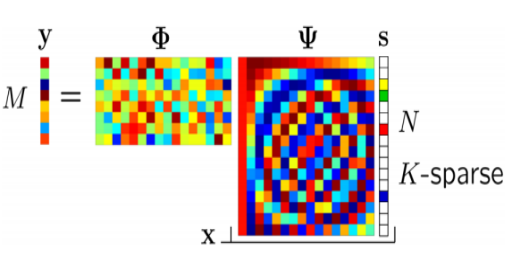
\includegraphics[scale=0.6]{CS1.png} 
\caption[Compressed sensing measurement process]{Measurement process in compressed sensing.}
\label{fig:csmea} 
\end{figure}
Figure \ref{fig:csmea} depicts the operation. Putting everything together each measurement $y_i$ is an $ M \times 1$ vector and $\{\phi\}_{i}^{T}$ representing the rows as a $ M \times N$ matrix $\mathbf{\Phi)}$, then the sampling process is
\begin{equation} \label{eq:signal2}
\hspace{3em} \hspace{3em} \hspace{3em} y = \Phi x = \Phi\Psi\alpha \hspace{3em}
\end{equation}    
from that one can see that the product of matrices $\Phi\Psi$ has size $ M \times N$ and the measurement matrix $\mathbf{\Phi}$ in independent from the signal $\mathbf{x)}$. The previous is important since the choice of the sensing matrix plays an important role for the reconstruction process, that is recovering $\mathbf{x}$ from measurements $\mathbf{y)}$. In particular, $\Phi$ and $\Psi$ should be incoherent. Coherence of two matrices is a measure that asserts the level of correlation of $\Phi$ and $\Psi$ and is computed as follows
\begin{equation} \label{eq:signal3}
\hspace{3em} \hspace{3em} \hspace{3em} \mu(\Phi,\Psi) = \max_{k,j}|<\phi_k,\psi_j>|  \hspace{3em}
\end{equation}   
the lower $\mu$ the more incoherent the matrices are and therefore the successful reconstruction of the original signal is more probable.

\subsection{Sensing Matrix and RIP}
The sensing matrix $\Phi$ should be chosen so that the number $M$ of its rows is larger than the number of nonzeros entries in the sparse signal $K$, that is $M \geq K$. Due to the fact that defining a number $K$ for natural signals is unknown, a constraint commonly referred as $restricted \enspace isometry \enspace property$ (RIP) \cite{candes2005decoding,candes2006stable,candes2008restricted} was proposed. It ensures that the matrix $\Phi$ retains the length of the k-sparse vectors and therefore the signal is not corrupted  by the transformation going from $\mathbf{x} \in R^N $ to $\mathbf{y} \in R^M $. The mathematical representation of RIP reads
\begin{equation} \label{eq:rip1}
\hspace{3em} \hspace{3em} \hspace{3em} (1-\delta_k)\Vert x \Vert_{l_2}^2 \leq \Vert \Phi x \Vert_{l_2}^2 \leq (1+\delta_k)\Vert x \Vert_{l_2}^2  \hspace{3em}
\end{equation}  
where $\delta_k$, referred to as $restricted \enspace isometry \enspace constant$, is the smallest number preserving the inequality for the matrix $\Phi$. \

Designing optimal sensing matrices goes beyond the scope of this thesis since the RIP and incoherence may be obtained with high probability by taking $\Phi$ as a random Gaussian matrix with independent and identically (iid) distributed elements\cite{candes2005signal} we will not devote more time for this topic. Particularly, we will use an iid Gaussian sensing matrix throughout the thesis unless otherwise specified.         

\subsection{Signal Recovery}
Even though RIP (\ref{eq:rip1}) and incoherence theoretically ensure that a K-sparse signal can be entirely described with only $M$ measurements, it is still necessary to restore the original signal $\mathbf{x}$. A great deal of algorithms alredy existing accomplish the recontruction process by reading the measurements $\mathbf{x}$, the matrix  $\Phi$ and solving an optimization problem. Concretely, most recovery algorithms try to find the best approximation $\hat{x} = \Psi x$ for some transform basis $\Psi$. It has been proved \cite{candes2006near,Donoho01} that the optimal solution for that problem is $\hat{x}$ with the smallest $l_0$ norm from measurements $y$ given by         
\begin{equation} \label{eq:minl0}
\hspace{3em} \hspace{3em} \hspace{3em} \hat{x} = arg \min_{x} \Vert \Psi x \Vert_0 \hspace{3em} s.t. \enspace \enspace y = \Phi x     \hspace{3em}
\end{equation}     
Nevertheless, the solution for \ref{eq:minl0} is NP-hard optimization problem that becomes numerically unstable and requires comprehensive computation. As a result, a convex relaxation was introduced and the $l_1$ norm is used instead reducing the problem to a linear program  of the form 
\begin{equation} \label{eq:minl1}
\hspace{3em} \hspace{3em} \hspace{3em} \hat{x} = arg \min_{x} \Vert \Psi x \Vert_1 \hspace{3em} s.t. \enspace \enspace y = \Phi x     \hspace{3em}
\end{equation}
This holds true because measurements $\mathbf{y}$ were taken using an iid Gausian sensing matrix and therefore a sucessful reconstruction is highly probable to occur \cite{Donoho01,candes2006robust}. Algorithms trying to solve this problem are dubbed iterative given the nature of convex optimization. Among state-of-the-art iterative algorithms one can find \cite{dong2014compressive,li2013efficient,metzler2014denoising} and they are used as a baseline to compare our results.  \

In this thesis we do not aim to find an iterative solution for the aforementioned optimization problem in equation \ref{eq:minl1}, instead we explore the promising capabilities of using deep learning for image processing tasks.

\section{Deep Learning}
Deep learning is a modern field of machine learning that makes used of deep neural networks in order to learn representations of data with several layers of abstraction. It has been an active research topic during recent years because they have achieved state-of-the-art results in image processing, video, speech and audio applications. It also solves the inability of traditional machine-learning methods to process plain raw data. Moreover, there is no need to have extensive experience in order to engineer features that transform data into useful representations or feature vectors that will ultimately allow the learning algorithm detect or classify the data. \

Deep-learning techniques, whether supervised or unsupervised, learn multiple level representations. Such representation are realized by simple but non-linear entities transforming the representation level by level into a higher and more abstract one. By stacking a sufficient number of such layers and by implementing a learning process, highly complex functions can be learned and accurately approximated. The main singularity of such layers is that the features are learned without much human intervention, that is clever engineering from a person with very specialized knowledge. Rather, those features are learned directly from the data.   \   

Because deep learning has proved to be effective in overcoming difficulties that have caused trouble in the artificial intelligence community for years and because more and more data is becoming available, it is highly expectated that deep learning will achieve more accomplishments in the near future \cite{lecun2015deep}.  

\subsection{Supervised learning} \label{sec:superv}
Supervised machine learning algorithms are trained using data composed of a group of inputs $\mathbf{x}$ and an analogous label $\mathbf{y}$. The main reason for this learning approach is to produce the most accurate mapping $f : \mathbf{x} \mapsto \mathbf{y} $ that is used to reproduce more labels. Examples for this kind of task are: classifying hand-written digits. Normally, we have a set of given hand-written numbers paired with the correct discrete class and we would like to train a model so that in the future we receive more hand-written digits and hopefully they will be correctly classified. On the other hand, we have a set of compressed measurements and its respective original images. In this case, we have a regression problem and our model will be trained so that new compressed measurements are fed into it and successful images are reconstructed.   

\subsection{Unsupervised learning} \label{sec:unsuperv}
Unlike supervised learning unsupervised learning is not given an explicit label $\mathbf{y}$. That means, the learning algorithm only has access to the input  $\mathbf{x}$ as the training data. The applications of unsupervised learning are: clustering, that is finding similarities on the data for a particular number of groups; density estimation, which aims to discover a distribution explaining the input data. Finally, unsupervised learning used to reduce the dimensionality of the input into a lower one that retains as much information as possible. \

In our case, we use the unsupervised approach to both learn a sensing matrix $\Phi$ and  reconstruct the image back to its original size from these measurement. 
        
\subsection{Neural Networks} \label{sec:NNs}
Neural networks (NN's), in the field of machine learning, are a mathematical attempt to approximate and estimate functions in the same way that many biological systems do. Even though its origins dates back to the 40's and 60's, they have found effective and active usage during recent years. There are three major concepts concerning NN's that one has to deal with to make use of them:  network architecture, activation function and network training.
\begin{figure}[tb] 
\centering 
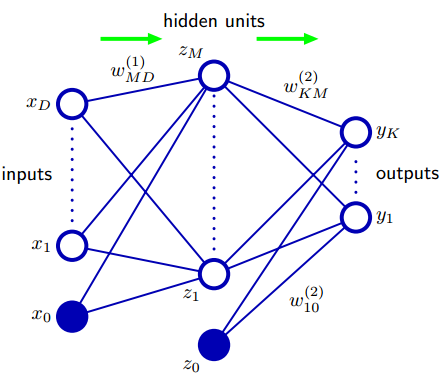
\includegraphics[scale=0.6]{NN1.png} 
\caption[Neural network example architecture]{A neural network takes $x_D$ inputs and gives $y_K$ outputs. Another important term is the number of hidden units which refers to the number of layers between the input and output layers. The term deep comes when the number of layers and its size grows larger. Most commonly $\omega_{MD}^{(i)}$ are called the weight parameters.}
\label{fig:NNim1} 
\end{figure} 
\begin{itemize}
\item \textbf{Network architecture} describes the number of parameters that build the network, the number of hidden layers and input and output size. Figure \ref{fig:NNim1} shows a node-like generalization of a  fully connected network architecture. The green arrows show how the information flows. Outputs $y_K$ are parameterize as a weighted sum of a predefined non-linear function $f$, $\omega$ and a bias $b$  
\begin{equation} \label{eq:paramNN}
\hspace{3em} \hspace{3em} \hspace{3em} y_K = f ( \sum_{i=1}^D \omega_i x_i + b  ) \enspace \hspace{3em}
\end{equation} 


Normally, $b$ is embedded into $\omega$ as an extra dimension to simplify its training and the representation becomes  

\begin{equation} \label{eq:paramNN}
\hspace{3em} \hspace{3em} \hspace{3em} y_K = f ( \sum_{i=1}^D \omega_i x_i  ) \enspace with \enspace  \omega \in \mathbb{R}^{d+1} \enspace \hspace{3em}
\end{equation}   

\item \textbf{Activation function} specifies the output of each neuron in the network according to a given input. Such input, is the product between $\omega$ and $x$ which is subsequently transformed by a function commonly referred to as nonlinearity because of its behavior. Most popular functions are plotted in Figures  sigmoid\ref{fig:Sigfun1}, tanh \ref{fig:tanhfun1} and more recently linear rectifier (ReLu) \ref{fig:ReLu1} \cite{glorot2011deep}. 
%\begin{equation} \label{eq:sigmoid}
%\hspace{3em} \hspace{3em} \hspace{3em} \sigma (x) = \frac{1}{1+e^{(-x)}} \enspace \enspace \hspace{3em}
%\end{equation} 
%\begin{equation} \label{eq:tanh}
%\hspace{3em} \hspace{3em} \hspace{3em} f (x) = \frac{2}{1+e^{(-2x)}}-1 \enspace %\enspace \hspace{3em}
%\end{equation} 
%\begin{equation} \label{eq:Relu}
%\hspace{3em} \hspace{3em} f (x) = \begin{cases} 0 & \text{for } x < 0 \\ x & \text{for } x \geqslant 0    \end{cases} \hspace{3em} or \hspace{3em} f (x) = \max %(0,x) \hspace{3em}
%\end{equation} 

\begin{figure}[tb] 
\centering 
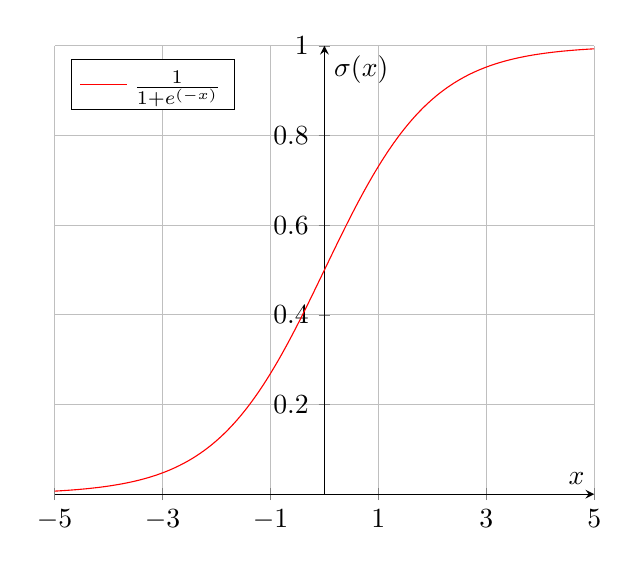
\begin{tikzpicture}  
\begin{axis}[
%   title={Sigmoid function},
    axis lines = center,
    legend pos=north west,
    xmin=-5, xmax=5,
    ymin=0, ymax=1,
    xtick={-5,-3,-1,0,1,3,5},
    xlabel = $x$,
    ylabel = {$ \sigma ( x )$},
    grid=major
]
%Below the red parabola is defined
\addplot [
    domain=-5:5, 
    samples=200, 
    color=red,
]
{(1)/(1+e^((-x)))}; 
\addlegendentry{$\frac{1}{1+e^{(-x)}}$}
\end{axis}
\end{tikzpicture}
\caption{Sigmoid function plot.}
\label{fig:Sigfun1} 
\end{figure}

\begin{figure}[tb] 
\centering 
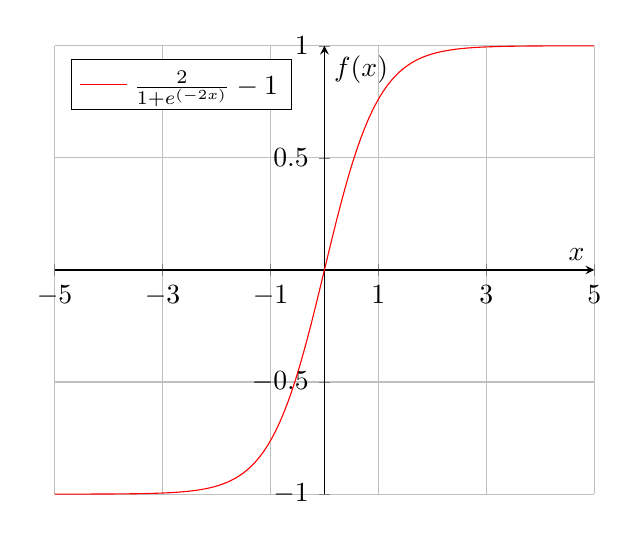
\begin{tikzpicture}  
\begin{axis}[
%   title={Sigmoid function},
    axis lines = center,
    legend pos=north west,
    xmin=-5, xmax=5,
    ymin=-1, ymax=1,
    xtick={-5,-3,-1,0,1,3,5},
    xlabel = $x$,
    ylabel = {$ f ( x )$},
    grid=major
]
%Below the red parabola is defined
\addplot [
    domain=-5:5, 
    samples=200, 
    color=red,
]
{tanh(x)}; 
\addlegendentry{$\frac{2}{1+e^{(-2x)}}-1$}
\end{axis}
\end{tikzpicture}
\caption{Tanh function plot.}
\label{fig:tanhfun1} 
\end{figure}

\begin{figure}[tb] 
\centering 
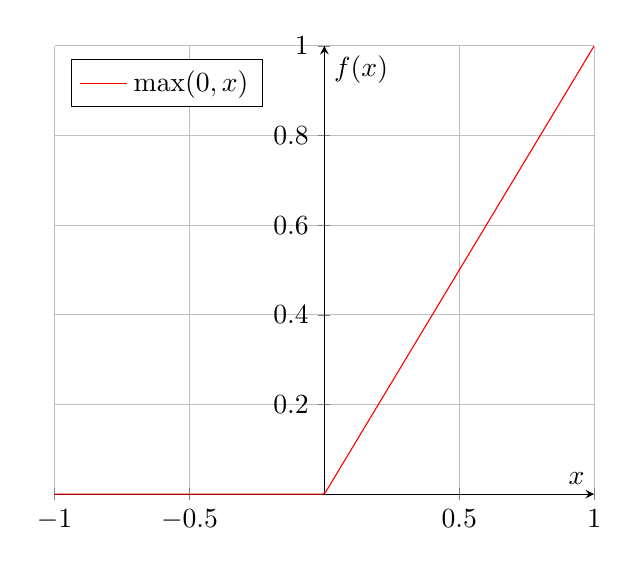
\begin{tikzpicture}  
\begin{axis}[
%   title={Sigmoid function},
    axis lines = center,
    legend pos=north west,
    xmin=-1, xmax=1,
    ymin=0, ymax=1,
    xtick={-1,-0.5,0,0.5,1},
    xlabel = $x$,
    ylabel = {$ f ( x )$},
    grid=major
]
%Below the red parabola is defined
\addplot [
    domain=-1:1, 
    samples=200, 
    color=red,
]
{max(0,x)}; 
\addlegendentry{$\max ( 0 , x)$}
\end{axis}
\end{tikzpicture}
\caption{ReLu function plot.}
\label{fig:ReLu1} 
\end{figure}


\item \textbf{Network training} is the process for learning the values of parameters $\omega$ of the network. The simplest way to solve the problem is by minimizing an error function, for example least squares error. That is achieved from a set of input vectors $x_n$, for $n = 1,...,N$, along with target vectors $y_n$. Using optimization theory we try to minimize 
\begin{equation} \label{eq:LS1}
\hspace{3em} \hspace{3em} \hspace{3em} E (w) = \frac{1}{2} \sum\limits_{n=1}^N \Vert f(x_n,w) - y_n\Vert^2 \enspace \enspace \hspace{3em}
\end{equation} 
thereby obtaining the optimum values for $\omega$. The actual minimization step uses of an algorithm called backpropagation, which is a method that computes the gradients by recursively applying chain rule. The error is computed by doing a forward pass in the network.  

\item \textbf{Chain rule} is a mathematical formula allowing to compute the gradient of a function with respect to another function. It is of importance for NN's because it helps find the derivative of the error between input and the output. Figure \ref{fig:CRim1} shows how the  gradient is computed through the network.

\begin{figure}[tb] 
\centering 
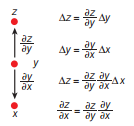
\includegraphics[scale=1.1]{CR1.png} 
\caption[Chain rule in neural networks]{Chain rule computation in the network.}
\label{fig:CRim1} 
\end{figure}

\item \textbf{Forward pass} is the process of taking the desired input and transforming it according to the current network parameters. The output is then compared with a desired target to obtain the error. Figure \ref{fig:FPim1} provides a graphical representation. 

\begin{figure}[tb] 
\centering 
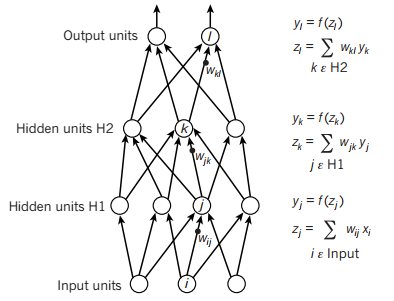
\includegraphics[scale=0.7]{FP1.png} 
\caption[Forward pass to compute error]{Forward pass is used to compute the predictions using the current values of weight patameters.}
\label{fig:FPim1} 
\end{figure}

\item \textbf{Backpropagation} is a technique that permits NN's to learn function approximations. Once the forward pass is carried out, the error is obtained evaluating loss function. Afterwards,  the gradient of the loss function with respect to the given input is recursively propagated through the network. The weights $\omega$ are updated by moving towards the minimum of the loss function. Figure \ref{fig:BPim1} depicts the process. The process of completing a forwards pass, error computation, loss gradient and backpropagation over all training examples is called epoch. 

\begin{figure}[tb] 
\centering 
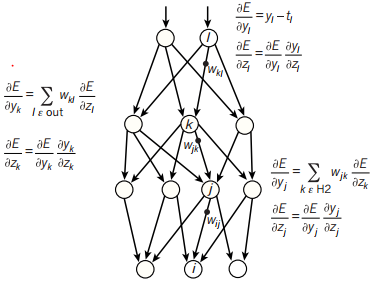
\includegraphics[scale=0.7]{BP1.png} 
\caption[Backpropagation process through the network]{After the error has been computed, it is backpropagated through the network updating $\omega$ parameters accordingly.}
\label{fig:BPim1} 
\end{figure} 	

\item \textbf{Gradient Descent (GD)} explain it!

\item \textbf{Stochastic gradient descent (SGD)} is used to find the minimum of a the loss function by iterating over each input example. Because of that, if the training examples are very large only one iteration would take a long time which would make the process slow. As a result, SGD is not scalable and limits its application to small datasets. Algorithm \ref{SDGalg} shows a generalization of how it is implemented. Another practical difficulty is to find a good learning rate $\alpha$. As a result, many algorithms try to adapt the learning on the go to avoid overshooting and allow for faster convergence.  

\begin{algorithm}
\caption{Stochastic Gradient Descen (SDG)}
\label{SDGalg}
\begin{algorithmic}[1]
    \Require  Learning rate $\alpha  $ 
    \Require $L ( \omega ) $: Loss function
    \Require $ \omega_0 $: Initial parameter values
    \State $t \leftarrow 0$ (Initialize timestep)
    \While{$\omega_t$ not converged}
        \State $t \leftarrow t+1$ 
        \State $g_t \leftarrow \nabla_{\omega} L_t ( \omega_{t-1} )$ (Gradient of loss function) 
        \State $\omega_t \leftarrow \omega_{t-1} - \alpha g_t $ (Update parameters)
    \EndWhile
    \State \Return $\omega_t $ (Resulting parameters)   
\end{algorithmic}
\end{algorithm}

\item \textbf{Mini-batch Stochastic gradient descent (SGD)} is the most commonly used algorithm for large neural networks because it overcomes the limitation of SGD for big datasets. Unlike SDG, it starts moving towards the minimum by just evaluating a small number of samples and updating the parameters accordingly. That is, not all training examples are used before $\omega$ values are changed. It introduces a new hyperparameter for the training specifiying the number $m$ of samples to be used during each iteration and it is referred to as batch size.        

\end{itemize} 



\subsection{Convolutional Neural Networks}
Convolutional Neural Networks (CNN's/ConvNets) are a subset of the previously described neural networks. They are also build of neurons that aim to learn weight parameters $\omega$ and bias parameters $b$ by performing dot products and normally followed by one of the afore mention nonllinear functions. The main difference, however, is that CNN's assume that the input are images that are convolved through the network during the forward pass and the number of parameters is lesser because the dot products are only computed in certain regions and not in the image as a whole.   

\subsubsection{CNN architecture}
In contrast with fully connected networks, the layers of CNN's are arranged in a 3D fashion seen as: width, height, depth. It differentiates in the sense that only a small subset of a layer connects to the one before it, thus reducing the number of neurons and encapsulating certain features in the input image as shown in  figure \ref{fig:CNNim1}. \

CNN's are assembled by interconnecting three different types of layers one after another: Convolutional Layer, Pooling Layer and Fully-Connected Layer. Optionally, the output of each layer is passed through the ReLu function \ref{fig:ReLu1}. 
\begin{itemize}
\item \textbf{Convolutional layer} is the main part composing a CNN. It computes the dot product between parameters $\omega$ and a small area of the input image. Its  functionality and output size are controlled by four hyperparameters: number of kernels or receptive fields $K$, size of kernel filters $F$, number of zero padding $P$ and stride $S$. Figure \ref{fig:CNNim2} shows the mechanism that  CNN's use, each channel of the input image is convolved with the filters generating an output.  \

\begin{figure}[tb] 
\centering 
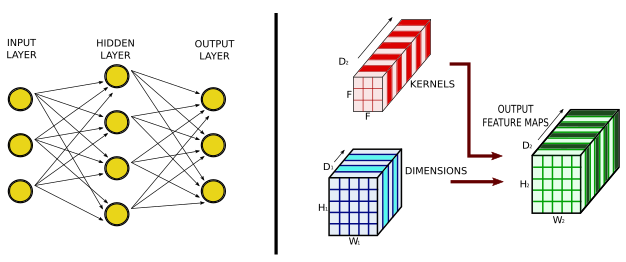
\includegraphics[scale=0.6]{CNN1.png} 
\caption[Fully connected network VS CNN]{\textbf{Left:} Fully connected network with 2 hidden layers. \textbf{Right} 3D (width, height, depth) arrangement of neurons. Each layer of the CNN carries out a 3D transformation on each channel (RGB in case of images). }
\label{fig:CNNim1} 
\end{figure}
\begin{figure}[tb] 
\centering 
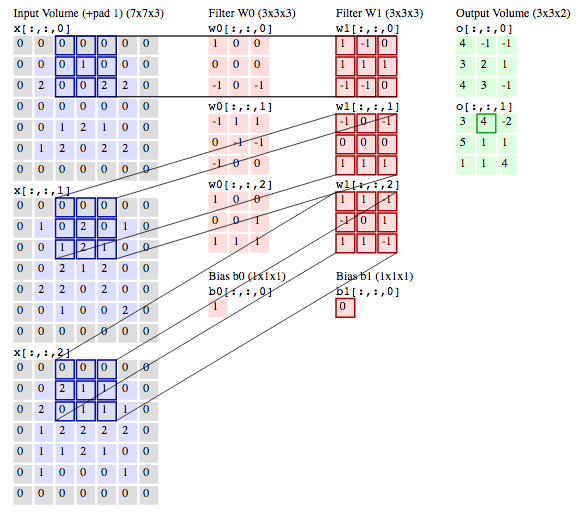
\includegraphics[scale=0.6]{CNN2.png} 
\caption[Convolution layer]{Example of a convolution layer in a 3D input with parameters Initial input volume $5 \times 5$, $K=2$, $F=3$, $S=2$ and $P=1$.}
\label{fig:CNNim2} 
\end{figure}


In general convolution layers have the following characteristics:
\begin{itemize}
\item Input size: \boldmath$W_1 \times H_1 \times D_1$
\item Hyperparaemters: Number of filters \boldmath$K$, filter size \boldmath$F$, stride \boldmath$S$ and zero padding \boldmath$P$.  
\item Output size: \boldmath$W_2 \times H_2 \times D_2$ where:
\begin{itemize} \label{sec:outCNN}
\item \boldmath$W_2 = ( W_1 - F + 2P) / S + 1 $
\item \boldmath$H_2 = ( H_1 - F + 2P) / S + 1 $
\item \boldmath$D_2 = K $
\end{itemize}
\end{itemize}

Sometimes it is necessary to preserve the original sizes of height and width, like in our case, a common setting to achieve that is by using these settings: $K =3$, $S =3$ and $P =3$.   

\item \textbf{Pooling layer} commonly used for classification purposes. Its main function is to reduce the spatial size, doing that allows to reduce the complexity of the network while maintaining information. In our experiments we do not make use of it. \

\item \textbf{Fully connected layer} is completely connected to all neurons in the previous layer, as in a regular neural network. It also makes networks grow lager and when used in CNN's they are commonly the last layer computing the final result for a type of classification. As with pooling layers we do not make use of it. 

\item \textbf{Activation function for CNN's} normally refers to a linear rectifier function ReLu \ref{fig:ReLu1}. It is explicitly given as another layer in the network and allows for efficient gradient propagation. It is very popular because not only is its computation easier than other activation functions like sigmoid \ref{fig:Sigfun1} or tahnh \ref{fig:tanhfun1} but, it also decreases the probability for observing vanishing gradients.

\end{itemize}

